% Sudut pada garis sejajar yang dipotong transversal
% Garis sejajar k (y=0) dan l (y=2); transversal t membentuk
% sudut 70 derajat terhadap garis mendatar.
% Titik potong bawah P(0,0); titik potong atas Q(0,73; 2),
% karena 2 * cot(70 derajat) = 0,73.
% Emas = sehadap (70 derajat), hijau = berseberangan dalam
% (70 derajat), merah = sepihak dalam (110 derajat).
\documentclass[tikz,border=8pt]{standalone}
\usepackage{tikz}
\definecolor{navy}{HTML}{14213D}
\definecolor{gold}{HTML}{C9A227}
\begin{document}
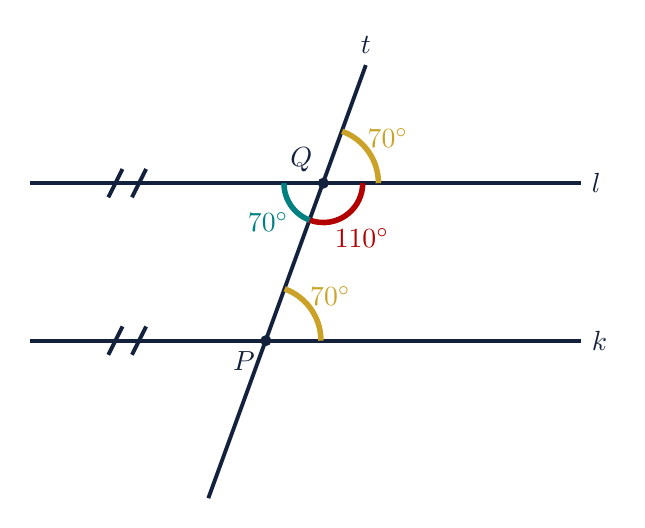
\begin{tikzpicture}[line width=1.4pt, color=navy]
  % Dua garis sejajar k dan l, dengan tanda sejajar
  \draw (-3,0) -- (4,0) node[right] {$k$};
  \draw (-3,2) -- (4,2) node[right] {$l$};
  \foreach \x in {-2,-1.7} {
    \draw (\x,-0.18) -- (\x+0.18,0.18);
    \draw (\x,1.82) -- (\x+0.18,2.18);
  }
  % Transversal t: naik 2, geser 0,73 (cot 70 derajat)
  \draw (-0.73,-2) -- (1.27,3.5) node[above] {$t$};

  % Titik potong
  \coordinate (P) at (0,0);
  \coordinate (Q) at (0.73,2);
  \fill (P) circle (2pt) (Q) circle (2pt);
  \node[below left] at (P) {$P$};
  \node[above left] at (Q) {$Q$};

  % Busur emas: sehadap, 70 derajat di kedua titik potong
  \draw[gold, line width=2pt] (0.7,0) arc[start angle=0, end angle=70, radius=0.7];
  \draw[gold, line width=2pt] (1.43,2) arc[start angle=0, end angle=70, radius=0.7];
  \node[gold] at (0.82,0.57) {$70^\circ$};
  \node[gold] at (1.55,2.57) {$70^\circ$};
  % Busur hijau: berseberangan dalam, 70 derajat
  \draw[teal, line width=2pt] (Q) ++(180:0.5)
    arc[start angle=180, end angle=250, radius=0.5];
  \node[teal] at (0.03,1.51) {$70^\circ$};
  % Busur merah: sepihak dalam, 110 derajat
  \draw[red!70!black, line width=2pt] (Q) ++(250:0.5)
    arc[start angle=250, end angle=360, radius=0.5];
  \node[red!70!black] at (1.22,1.30) {$110^\circ$};
\end{tikzpicture}
\end{document}
